\documentclass[11pt]{article}
\usepackage{graphicx}
\usepackage{subcaption}
\usepackage{tabularx}
\usepackage{float}
\usepackage{listings}
\usepackage{caption}
\usepackage{amsmath}
\usepackage{algorithm}
\usepackage{algpseudocode}
\usepackage{amssymb}
\usepackage{listings}
\usepackage[inline]{enumitem}
\usepackage{xcolor}
\usepackage[top = 0.7in,bottom = 0.8in, left = 0.8in, right = 0.8in]{geometry} 
\usepackage{hyperref}
%New colors defined below
\definecolor{codegreen}{rgb}{0,0.6,0}
\definecolor{codegray}{rgb}{0.5,0.5,0.5}
\definecolor{codepurple}{rgb}{0.58,0,0.82}
\definecolor{backcolour}{rgb}{0.95,0.95,0.92}

%Code listing style named "mystyle"
\lstdefinestyle{mystyle}{
  backgroundcolor=\color{backcolour},   commentstyle=\color{codegreen},
  keywordstyle=\color{magenta},
  numberstyle=\tiny\color{codegray},
  stringstyle=\color{codepurple},
  basicstyle=\ttfamily\footnotesize,
  breakatwhitespace=false,         
  breaklines=true,                 
  captionpos=b,                    
  keepspaces=true,                 
  numbers=left,                    
  numbersep=5pt,                  
  showspaces=false,                
  showstringspaces=false,
  showtabs=false,                  
  tabsize=2
} 
\lstset{style=mystyle}

\title{\textbf{SC627 : Assignment 2}}
\author{\textbf{Adityaya Dhande}   \hspace{8mm} \textbf{210070005}}
\date{}
\begin{document}
\maketitle
\noindent
\section{Approach}
I have implemented an artificial potential field algorithm, with low potential for points close to the goal and high potential for points close to obstacles. 


Let $(x, y)$ be the position of the robot and $(x_g, y_g)$ be the goal. The attractive potential and force respectively are given by 
\begin{equation*}
    U_a = \frac{1}{2} K_a \{(x - x_g)^2 + (y-y_g)^2\} \hspace{1cm} -\nabla U_a = K_a \begin{bmatrix}
        (x_g - x) & (y_g - y)
    \end{bmatrix} 
\end{equation*}
I imposed an upper bound on the magnitude of the gradient which comes into effect when the distance between the robot and the goal is greater than $d^*_g$.
The gradient becomes,
 $$  \frac{d^*_g}{d} \nabla U_a \text{ for } d > d^*_g, \text{ where } d = \sqrt{(x-x_g)^2 + (y-y_g)^2}$$
 
The repulsive potential and force is calculated separately for each ray of the laser-scanner and adding the individual components. 
\begin{equation*}
    U_r^i = \frac{1}{2} K_r \{
        \frac{1}{d} - \frac{1}{d^*_o}
    \}^2 \text{ for } d < d^*_o, \text{ and } U_r^i = 0 \text{ for }  d \geq d^*_o
\end{equation*}
Where $d$ is the distance returned by the laser scanner. For $d < d^*_o$ the gradient of the potential is,
$$ \nabla U_r^i = - K_r \{\frac{1}{d} - \frac{1}{d^*_o}\}\frac{1}{d^2} \begin{bmatrix}
    \cos(\theta) & \sin(\theta)
\end{bmatrix} $$
$\theta$ is the orientation of the corresponding laser in the inertial frame. Finally, we have
$$ U_r = \sum_i U_r^i \text{ and } \nabla U_r = \sum_i U_r^i$$

In the \textbf{final implementation} I used $U_r^i = \frac{1}{2} K_r \{
    \frac{1}{d} - \frac{1}{d^*_o}
\}^4 \text{ for } d < d^*_o, \text{ and } U_r^i = 0 \text{ for }  d \geq d^*_o$

\subsection*{Generating target movement direction and speed}
Initially I summed up the gradients of attractive and repulsive potentials, and used the magnitude and direction of this gradient vector to 
set the target speed(by scaling the magnitude) and direction respectively. Following this approach I encountered some problems with local minima, where the robot entered an infinite loop of going back and forth or along a certain loop at an undesirable position which was not the goal. Also there were oscillations
when the robot moved in between obstacles to reach the goal. It oscillated back and forth between the obstacles. 
$$v^* = K_v \Vert V\Vert \text{ and } \psi^* = \arctan(V_x, V_y) \text{ where } V = (V_x, V_y) = \nabla U_a + \nabla U_r$$ 
After looking at \hyperref[foo]{1}, I found a solution to this problem. I simplified my initial approach and switched to a ``search" like algorithm. 
I evaluate the potential at $N$ points evenly spaced on a circle of radius $r$ and centered at the robot. I then move in the direction of least potential among the $N$ points. This has solved the problem of 
local minima and oscillations. Though it needs more computation compared to the gradient approach, it 
is still practically feasible and works in my implementation.
\begin{figure}[H]
    \begin{center}
        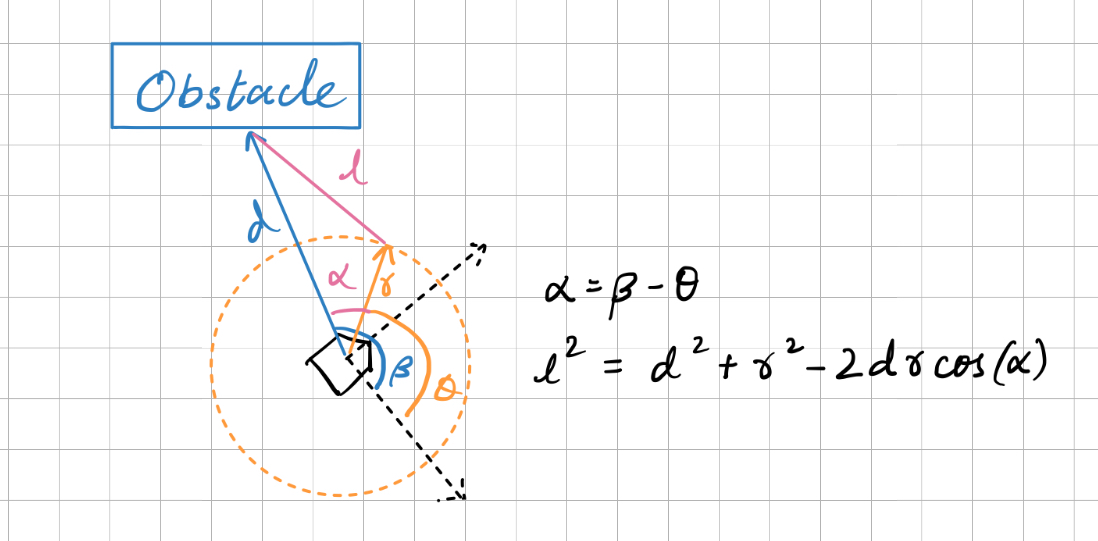
\includegraphics[width=0.6\linewidth]{images/Apf.png}
        \caption*{This figure shows how I evaluate the potential at these new points on the circle around the robot
        }
    \end{center}
\end{figure}
\subsection*{Moving in target direction and speed}
I am handling the speed control of the robot by directly giving the target speed to the turtle bot in the $x$ direction of the body frame. I am doing this 
by sending \texttt{Twist.linear.x} as the desired speed, and other components 0.

To handle the heading error however, we have to control it using the angular velocity. I defined an error in the orientation of the robot as the difference between the current orientation and the target direction. 
I am using a PD controller till the error reduces within some tolerance. The robot does not move till this happens, and while it is moving a P controller is active to take care of the residual error (which is within the tolerance). 

I made a slight improvement to the controller described above by exploiting the 
ability of turtle bot to move backward and forward. When the error in heading angle is more than $\pi/2$
in a certain direction, I make the robot turn $\pi - \text{error}$, in the opposite direction and give it a negative linear velocity.

\section{Choice of potential}
For the artificial potential function method to work, the goal should have the least potential and obstacles should have high potential, with no local minimas in the potential function. The potential functions I used are described in section 1. They satisfy the requirements for this algorithm. I used them 
after taking inspiration from \hyperref[foo]{1} and the planner was working with that choice. I tried a few modifications for the repulsive potential functions for better repulsion of obstacles (repulsions of the order $1/d^4$). This was to mainly deal with the dynamic obstacles as the robot would not get enough time to maneuver out of the path of the obstacle if it detected the obstacle only when it was close to the robot.
The fourth order repulsion increases the effect of repulsion at farther distances from the obstacle and it performed better in the simulation. However I had to increase the attractive potential also to remove some local minima which got created. 
\section{Limitations and possible improvements}
I tested the algorithm on hardware, while moving around, simulating an obstacle. It worked well for normal and slow walking speeds while I was walking in front of the turtlebot.
 
The code can be made efficient by combining both the algorithms that I mentioned which would involve calculating the gradient first and then 
moving in the direction of least potential amongst points around around the gradient. The gradient is close to the direction we obtain by using the ``search'' based algorithm so combining the two in this way is beneficial.

Also this implementation is not robust to dynamic obstacles. It is able to avoid slow moving obstacles but it is not able to 
avoid colliding with fast moving obstacles on some occasions (especially head on collisions).
This is because of the physical constraints on the robot which limit its angular and linear velocities, and also 
inability to measure the velocity of an obstacle using the laser scanner. 
\section{Running the code}
\texttt{planner.py} takes goal in the form of command line arguments. It can be executed using
 \\ \texttt{rosrun \${package\_name} planner.py \$goal\_x \$goal\_y} 
\section{References}
\begin{enumerate}
    \item \label{foo}Sun J, Liu G, Tian G, Zhang J. Smart Obstacle Avoidance Using a Danger Index for a Dynamic Environment. Applied Sciences. 2019; 9(8):1589
\end{enumerate}
\end{document}